\vspace{-0.5em}
Novel way of updating weight matrices in a lower rank
\begin{enumerate}
    \item Decompose the original weight matrix into U, S, V matrices using SVD
    \item Split U, S, V into smaller training (using the highest r singular values) and reconstruction (rank d) matrices
    \item Reconstruct the original model without using the trainable part
    \item Train the lower rank U and V matrices
    \item During forward pass, reconstruct trainable U, S, V and add it to the original matrix
\end{enumerate}
\vspace{-30pt}
\begin{figure}
    \centering
    \includesvg[width=\textwidth]{siva}
    \caption{SiVA diagram}
\end{figure}
\begin{itemize}
    \item Unlike LoRA, it has no random or zero initialization 
    \item Approximates full fine-tuning as close as possible
    \item Represents the whole weight matrix and applies updates over it in a lower rank
\end{itemize}
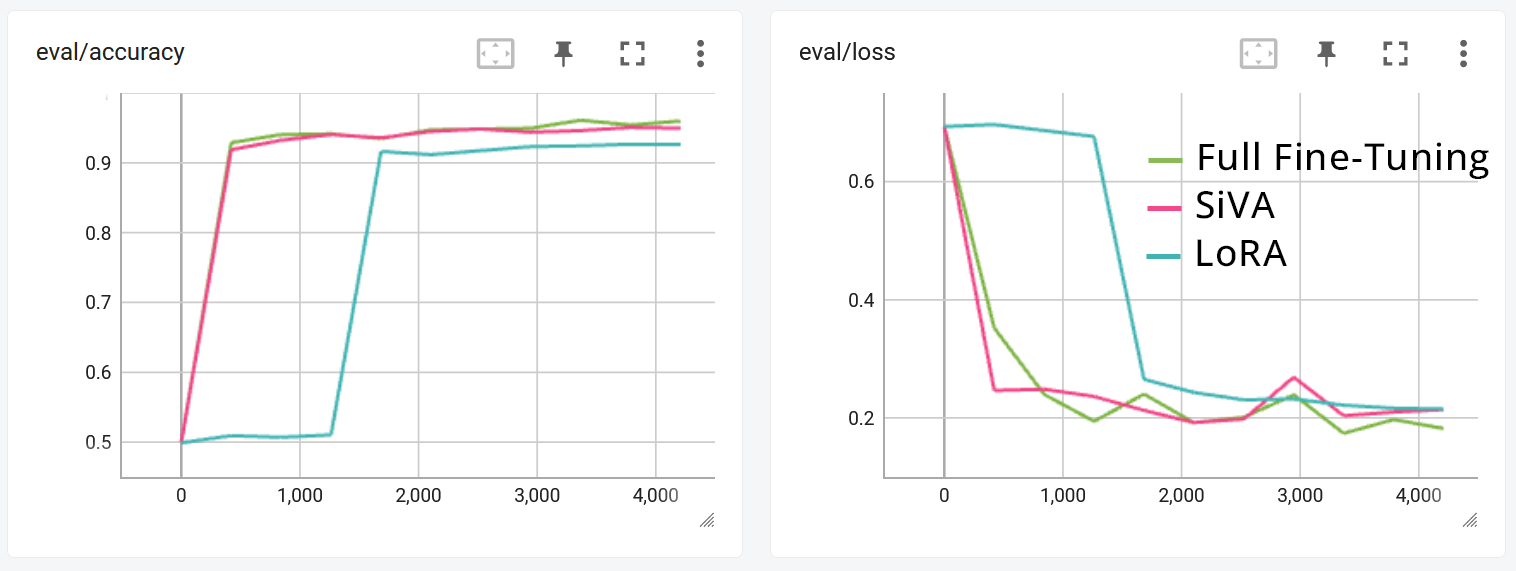
\includegraphics[width=\textwidth]{assets/images/siva-lora-comparison-3.png}
\captionof{figure}{Full fine-tuning, SiVA, and LoRA comparison with the same hyperparameters \& initialization}